%\documentclass[hyperref={pdfpagelabels=false},slidetop,9pt]{beamer}
\documentclass[slidetop,8pt]{beamer}
\usepackage[T1]{fontenc}
\usepackage[utf8]{inputenc}
\newcommand{\id}{54}
\newcommand{\nom}{Liaisons mécaniques}
\newcommand{\sequence}{04}
\newcommand{\num}{01}
\newcommand{\type}{TP}
\newcommand{\descrip}{Modélisation d'un solide. Comportement des liaisons mécaniques. Modéliser les mécanismes du laboratoire par un schéma cinématique, paramétré.}
\newcommand{\competences}{A3-C4: Analyse d'architecture et de comportement \\ &  Mod1-C1: Isolement d'un solide ou d'un système de solides \\ &  Mod2-C10-1: Modèle de solide indéformable \\ &  Mod2-C11: Modélisation géométrique et cinématique des mouvements entre solides indéformables \\ &  Mod2-C12: Modélisation cinématique des liaisons entre solides \\ &  Mod2-C15: Modélisation des actions mécaniques \\ &  Rés-C6: Utilisation d'un solveur ou d'un logiciel multi physique \\ &  Com1-C1: Différents descripteurs introduits dans le programme \\ &  Com2-C4: Outils de communication}
\newcommand{\nbcomp}{9}
\newcommand{\systemes}{Plateforme Stewart}
\newcommand{\systemessansaccent}{Plateforme Stewart}
\newcommand{\ilot}{2}
\newcommand{\ilotstr}{02}
\newcommand{\dossierilot}{\detokenize{Ilot_02 Plateforme Stewart}}
\newcommand{\imageun}{Plateforme}

\newcommand{\urlsysteme}{\href{https://www.costadoat.fr/systeme/57}{Ressources système}}
\newcommand{\matlabsimscape}{\href{https://github.com/Costadoat/Sciences-Ingenieur/raw/master/Systemes/Plateforme Stewart/Plateforme_Stewart_Simscape.zip}{Modèle Simscape}}
\newcommand{\solidworks}{\href{https://github.com/Costadoat/Sciences-Ingenieur/raw/master/Systemes/Plateforme Stewart/Plateforme_Stewart_Solidworks.zip}{Modèle Solidworks}}
\newcommand{\edrawings}{\href{https://github.com/Costadoat/Sciences-Ingenieur/raw/master/Systemes/Plateforme Stewart/Plateforme_Stewart.EASM}{Modèle eDrawings}}
\newcommand{\test}{Stewart_param1}
\newcommand{\testi}{Stewart_param2}
\newcommand{\testii}{Stewart_param3}
\newcommand{\testiii}{Stewart_param4}
\newcommand{\testiiii}{Stewart_euler}
\usepackage{etex}
\usepackage{tikz}
\usepackage[european]{circuitikz}
\usepackage{pgf}
\usepackage[all]{xy}
\usepackage{pgfpages}
\usepackage{graphbox}
\usepackage{pdfpages}
\usepackage[adobe-utopia]{mathdesign}
\usepackage{ifthen}
\usepackage{cancel}
\usepackage{framed}
\usepackage{subfig}
\usepackage{tabularx}
\usepackage{setspace}
\usepackage{soul}
\usepackage{schemabloc}
\usepackage{eqnarray}
\usepackage[dot, phantomtext]{dashundergaps}
\usepackage{media9}
\usepackage{multimedia}
\usepackage{textcomp}

\author{Renaud Costadoat}
\institute{Lycée Dorian}

\usepackage{multido}
\usepackage{multirow}
\usepackage{multicol} % Portions de texte en colonnes
\usepackage{flafter}%floatants après la référence

\usepackage{color}
\usepackage{xcolor}
\usepackage{colortbl}

\usepackage[gen]{eurosym}
\usepackage{tikz}
%\usepackage{pstricks,pst-node,pst-tree,pst-solides3d}
\usepackage{lmodern}
\usepackage[francais]{babel}
\usepackage{pslatex}
\usetheme{renaud}
\usepackage{times}
\usepackage{amsmath}
\usepackage{verbatim}
\usepackage{moreverb}
%\usetikzlibrary{arrows,shapes}
\usepackage{graphicx}
\usepackage{psfrag}
\usepackage{wrapfig}
\usepackage{etoolbox}

\definecolor{gris25}{gray}{0.75}
\definecolor{bleu}{RGB}{18,33,98}
\definecolor{bleuf}{RGB}{42,94,171}
\definecolor{bleuc}{RGB}{231,239,247}
\definecolor{rougef}{RGB}{185,18,27}
\definecolor{rougec}{RGB}{255,188,204}%255,230,231
\definecolor{vertf}{RGB}{103,126,82}
\definecolor{vertc}{RGB}{220,255,191}

\setlength\parindent{24pt}
\parskip 7.2pt
\parindent 8pt

\newenvironment{rem}[1][\hsize]%
{%
    \def\FrameCommand
   {%
\rotatebox{90}{\textit{\textsf{Remarque}}} 
       {\color{bleuf}\vrule width 3pt}%
       \hspace{0pt}%must no space.
       \fboxsep=\FrameSep\colorbox{bleuc}%
  }%
    \MakeFramed{\hsize#1\advance\hsize-\width\FrameRestore}%
}%
{\endMakeFramed}%


\newenvironment{savoir}[1][\hsize]%
{%
    \def\FrameCommand
    {%
\rotatebox{90}{\textit{\textsf{Savoir}}} 
        {\color{bleuf}\vrule width 3pt}%
        \hspace{0pt}%must no space.
        \fboxsep=\FrameSep\colorbox{bleuc}%
    }%
    \MakeFramed{\hsize#1\advance\hsize-\width\FrameRestore}%
}%
{\endMakeFramed}%

\newenvironment{prob}[1][\hsize]%
{%
    \def\FrameCommand%
    {%
\rotatebox{90}{\textit{\textsf{Problematique}}} 
        {\color{rougef}\vrule width 3pt}%
        \hspace{0pt}%must no space.
        \fboxsep=\FrameSep\colorbox{rougec}%
    }%
    \MakeFramed{\hsize#1\advance\hsize-\width\FrameRestore}%
}%
{\endMakeFramed}%

\newenvironment{obj}[1][\hsize]%
{%
    \def\FrameCommand%
    {%
\rotatebox{90}{\textit{\textsf{Objectif}}} 
        {\color{vertf}\vrule width 3pt}%
        \hspace{0pt}%must no space.
        \fboxsep=\FrameSep\colorbox{vertc}%
    }%
    \MakeFramed{\hsize#1\advance\hsize-\width\FrameRestore}%
}%
{\endMakeFramed}%

\newenvironment{defi}[1][\hsize]%
{%
    \def\FrameCommand%
    {%
\rotatebox{90}{\textit{\textsf{Definition}}} 
        {\color{bleuf}\vrule width 3pt}%
        \hspace{0pt}%must no space.
        \fboxsep=\FrameSep\colorbox{rougec}%
    }%
    \MakeFramed{\hsize#1\advance\hsize-\width\FrameRestore}%
}%
{\endMakeFramed}%


\newenvironment{hypo}[1][\hsize]%
{%
    \def\FrameCommand%
    {%
\rotatebox{90}{\textit{\textsf{Hypothèse\\}}} 
        {\color{bleuf}\vrule width 3pt}%
        \hspace{0pt}%must no space.
        \fboxsep=\FrameSep\colorbox{bleuc}%
    }%
    \MakeFramed{\hsize#1\advance\hsize-\width\FrameRestore}%
}%
{\endMakeFramed}%


\newenvironment{prop}[1][\hsize]%
{%
    \def\FrameCommand%
    {%
\rotatebox{90}{\textit{\textsf{Propriété}}} 
        {\color{bleuf}\vrule width 3pt}%
        \hspace{0pt}%must no space.
        \fboxsep=\FrameSep\colorbox{bleuc}%
    }%
    \MakeFramed{\hsize#1\advance\hsize-\width\FrameRestore}%
}%
{\endMakeFramed}%

\newenvironment{props}[1][\hsize]%
{%
    \def\FrameCommand%
    {%
\rotatebox{90}{\textit{\textsf{Propriétés}}} 
        {\color{bleuf}\vrule width 3pt}%
        \hspace{0pt}%must no space.
        \fboxsep=\FrameSep\colorbox{bleuc}%
    }%
    \MakeFramed{\hsize#1\advance\hsize-\width\FrameRestore}%
}%
{\endMakeFramed}%

\newenvironment{exemple}[1][\hsize]%
{%
    \def\FrameCommand%
    {%
\rotatebox{90}{\textit{\textsf{Exemple}}} 
        {\color{vertf}\vrule width 3pt}%
        \hspace{0pt}%must no space.
        \fboxsep=\FrameSep\colorbox{vertc}%
    }%
    \MakeFramed{\hsize#1\advance\hsize-\width\FrameRestore}%
}%
{\endMakeFramed}%

\newenvironment{resultat}[1][\hsize]%
{%
    \def\FrameCommand%
    {%
\rotatebox{90}{\textit{\textsf{Résultat}}} 
        {\color{rougef}\vrule width 3pt}%
%        {\color{bleuf}\vrule width 3pt}%
        \hspace{0pt}%must no space.
        \fboxsep=\FrameSep\colorbox{rougec}%
    }%
    \MakeFramed{\hsize#1\advance\hsize-\width\FrameRestore}%
}%
{\endMakeFramed}%

\newenvironment{methode}[1][\hsize]%
{%
    \def\FrameCommand%
    {%
\rotatebox{90}{\textit{\textsf{Méthode\\}}} 
        {\color{rougef}\vrule width 3pt}%
        \hspace{0pt}%must no space.
        \fboxsep=\FrameSep\colorbox{rougec}%
    }%
    \MakeFramed{\hsize#1\advance\hsize-\width\FrameRestore}%
}%
{\endMakeFramed}%

\newenvironment{theo}[1][\hsize]%
{%
    \def\FrameCommand%
    {%
\rotatebox{90}{\textit{\textsf{Théorème\\}}} 
        {\color{rougef}\vrule width 3pt}%
        \hspace{0pt}%must no space.
        \fboxsep=\FrameSep\colorbox{rougec}%
    }%
    \MakeFramed{\hsize#1\advance\hsize-\width\FrameRestore}%
}%
{\endMakeFramed}%

\newenvironment{warn}[1][\hsize]%
{%
    \def\FrameCommand%
    {%
\rotatebox{90}{\textit{\textsf{Attention\\}}} 
        {\color{rougef}\vrule width 3pt}%
        \hspace{0pt}%must no space.
        \fboxsep=\FrameSep\colorbox{rougec}%
    }%
    \MakeFramed{\hsize#1\advance\hsize-\width\FrameRestore}%
}%
{\endMakeFramed}%

% \usepackage{pstricks}
%\usepackage{minitoc}
% \setcounter{minitocdepth}{4}

\setcounter{tocdepth}{2}

% \mtcselectlanguage{french} 

%\usepackage{draftcopy}% "Brouillon"
% \usepackage{floatflt}
\usepackage{psfrag}
%\usepackage{listings} % Permet d'insérer du code de programmation
\renewcommand{\baselinestretch}{1.2}

% Changer la num�rotation des figures :
% ------------------------------------
% \makeatletter
% \renewcommand{\thefigure}{\ifnum \c@section>\z@ \thesection.\fi
%  \@arabic\c@figure}
% \@addtoreset{figure}{section}
% \makeatother
 


%%%%%%%%%%%%
% Définition des vecteurs %
%%%%%%%%%%%%
 \newcommand{\vect}[1]{\overrightarrow{#1}}

%%%%%%%%%%%%
% Définition des torseusr %
%%%%%%%%%%%%

 \newcommand{\torseur}[1]{%
\left\{{#1}\right\}
}

\newcommand{\torseurcin}[3]{%
\left\{\mathcal{#1} \left(#2/#3 \right) \right\}
}

\newcommand{\torseurstat}[3]{%
\left\{\mathcal{#1} \left(#2\rightarrow #3 \right) \right\}
}

 \newcommand{\torseurc}[8]{%
%\left\{#1 \right\}=
\left\{
{#1}
\right\}
 = 
\left\{%
\begin{array}{cc}%
{#2} & {#5}\\%
{#3} & {#6}\\%
{#4} & {#7}\\%
\end{array}%
\right\}_{#8}%
}

 \newcommand{\torseurcol}[7]{
\left\{%
\begin{array}{cc}%
{#1} & {#4}\\%
{#2} & {#5}\\%
{#3} & {#6}\\%
\end{array}%
\right\}_{#7}%
}

 \newcommand{\torseurl}[3]{%
%\left\{\mathcal{#1}\right\}_{#2}=%
\left\{%
\begin{array}{l}%
{#1} \\%
{#2} %
\end{array}%
\right\}_{#3}%
}

 \newcommand{\vectv}[3]{%
\vect{V\left( {#1} \in {#2}/{#3}\right)}
}


\newcommand{\vectf}[2]{%
\vect{R\left( {#1} \rightarrow {#2}\right)}
}

\newcommand{\vectm}[3]{%
\vect{\mathcal{M}\left( {#1}, {#2} \rightarrow {#3}\right)}
}


 \newcommand{\vectg}[3]{%
\vect{\Gamma \left( {#1} \in {#2}/{#3}\right)}
}

 \newcommand{\vecto}[2]{%
\vect{\Omega\left( {#1}/{#2}\right)}
}

\newcommand{\reponse}[1][4]
{
\multido{}{#1}
{
\begin{center}
\makebox[0.9\linewidth]{\dotfill} \end{center}
}}


% }$$\left\{\mathcal{#1} \right\}_{#2} =%
% \left\{%
% \begin{array}{c}%
%  #3 \\%
%  #4 %
% \end{array}%
% \right\}_{#5}}


%  ------------------------------------------
% | Modification du formatage des sections : | 
%  ------------------------------------------

% Grands titres :
% ---------------

\newcommand{\titre}[1]{%
\begin{center}
      \bigskip
      \rule{\textwidth}{1pt}
      \par\vspace{0.1cm}
      
      \textbf{\large #1}
      \par\rule{\textwidth}{1pt}
    \end{center}
    \bigskip
  }

% Supprime le numéro du chapitre dans la numérotation des sections:
% -----------------------------------------------------------------
\makeatletter
\renewcommand{\thesection}{\@arabic\c@section}
\makeatother


% \titleformat{\chapter}[display]
% {\normalfont\Large\filcenter}
% {}
% {1pc}
% {\titlerule[1pt]
%   \vspace{1pc}%
%   \Huge}[\vspace{1ex}%
% \titlerule]


%%%% Chapitres Comme PY Pechard %%%%%%%%%
% numéro du chapitre
\DeclareFixedFont{\chapnumfont}{OT1}{phv}{b}{n}{80pt}
% pour le mot " Chapitre "
\DeclareFixedFont{\chapchapfont}{OT1}{phv}{m}{it}{40pt}
% pour le titre
\DeclareFixedFont{\chaptitfont}{T1}{phv}{b}{n}{25pt}

\definecolor{gris}{gray}{0.75}
\setbeamertemplate{section in toc}[sections numbered]

\newlength{\RoundedBoxWidth}
\newsavebox{\GrayRoundedBox}
\newenvironment{GrayBox}[1][\dimexpr\textwidth-4.5ex]%
   {\setlength{\RoundedBoxWidth}{\dimexpr#1}
    \begin{lrbox}{\GrayRoundedBox}
       \begin{minipage}{\RoundedBoxWidth}}%
   {   \end{minipage}
    \end{lrbox}
    \begin{center}
    \begin{tikzpicture}%
       \draw node[draw=bleuf,fill=bleuc,rounded corners,%
             inner sep=2ex,text width=\RoundedBoxWidth]%
             {\usebox{\GrayRoundedBox}};
    \end{tikzpicture}
    \end{center}}
    
\ifdef{\prive}{\pgfpagesuselayout{2 on 1}[a4paper,border shrink=0mm]}
\ifdef{\prive}{\setbeamertemplate{navigation symbols}{}}
\setbeamertemplate{itemize item}[ball]
%\setbeamertemplate{blocks}[rounded]%[shadow=true]
\setbeamercolor{block title}{fg=white,bg=grisf}        % titre block normal 
\setbeamercolor{block body}{fg=grisf,bg=grisc!50}      % corps block normal
\setbeamercolor{block body alerted}{fg=white,bg=warning}   % idem pour un block alerte

\title{\nom}
\date{S\sequence \ - \type\num}

\begin{document}
\shorthandoff{:!}
\bibliographystyle{abbrvnat-fr}

\usebackgroundtemplate%
{%
    \centering
\includegraphics[width=\paperwidth]{../../img/fond2}%
}

{
\setbeamertemplate{navigation symbols}{}
\setbeamertemplate{headline}[pagetitre]
\setbeamertemplate{footline}[pagetitre]
\usebackgroundtemplate{\centering
\includegraphics[width=\paperwidth]{../../img/fond}}
\frame{\titlepage}
}



\section{Introduction}

{\frame{
\frametitle{Introduction}

\begin{savoir}
Vous êtes capables :
\begin{itemize}
 \item donner certaines caractéristiques d'un matériau.
\end{itemize}
\end{savoir}

\begin{prob}
Vous devez êtes capables de choisir un procédé de fabrication en fonction:
\begin{itemize}
 \item de la géométrie d'une pièce,
 \item de son matériau,
 \item de la production associée à la pièce.
\end{itemize}
\end{prob}
}}


{\frame{
\frametitle{Plan}
  \tableofcontents[currentsection]
}}

{\frame{
\frametitle{Propriétés et définitions}

\begin{defi}
Le \textbf{moulage} ou \textbf{fonderie} consiste à réaliser des pièces brutes par coulée du métal en fusion dans un moule (représentant l'empreinte de la pièce à obtenir). Le métal en se solidifiant, reproduit les contours et dimensions de l'empreinte du moule. 
\end{defi}

\begin{rem}
\begin{itemize}
 \item \textbf{Utilisation}: Cette technique permet de produire des pièces de formes complexes, la série des pièces est identique et elle permet l'obtention de pièces massives telles que bâtis, volants, etc...
 \item \textbf{Matériaux}: La majorité des matériaux (métalliques et non métalliques) peuvent être moulés.
\end{itemize}
\end{rem}
}}

{\frame{
\frametitle{Déformation plastique}

Le forgeage utilise la déformation plastique des métaux.

\begin{center}
 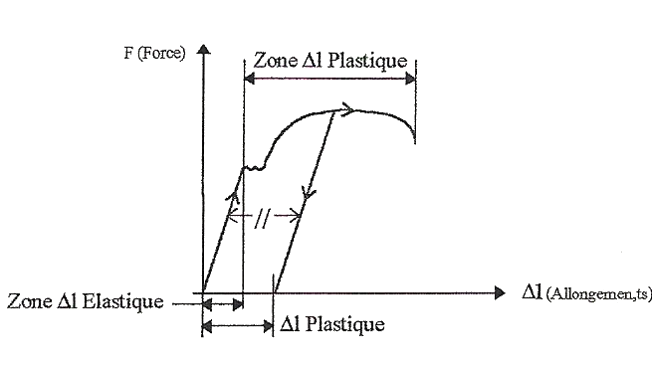
\includegraphics[width=0.9\linewidth]{img/Picture1}
\end{center}
}}

{\frame{
\frametitle{Évolution des caractéristiques matériaux (T°)}

Tout les métaux ne nécessitent pas les mêmes conditions afin d'être forgés.

\begin{center}
\begin{minipage}{0.45\linewidth}
\begin{tabular}{|p{0.25\linewidth}|p{0.35\linewidth}|p{0.35\linewidth}|}
\hline
\textbf{Alliages} & \textbf{Températures (°C)} & \textbf{Allongement (\%)} \\
\hline
Aluminium & 150 & 17-31 \\
 & 400 & 110-160 \\
\hline
Cuivre & 20 & 35-65 \\
 & 700 & >60 \\
\hline
Fer & 20 & 45-55 \\
 & 800 & 65-105 \\
 \hline
\end{tabular}
\end{minipage}\hfill
\begin{minipage}{0.45\linewidth}
 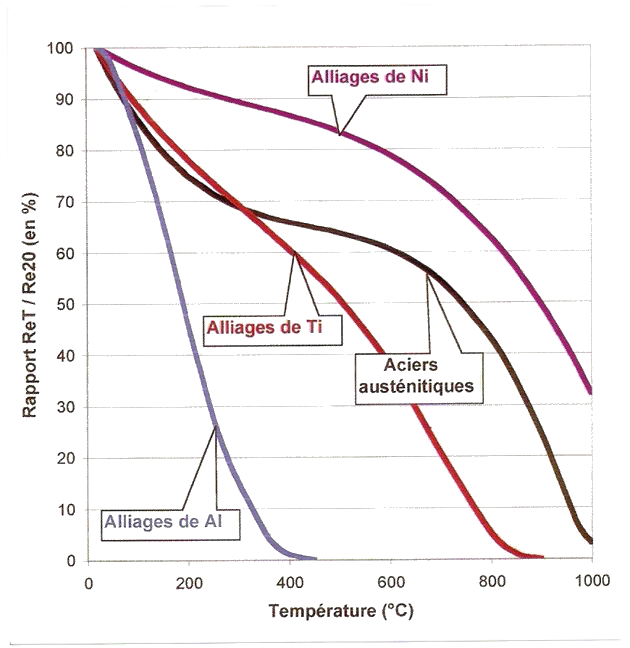
\includegraphics[width=0.9\linewidth]{img/Picture2}
\end{minipage}
\end{center}
}}

{\frame{
\frametitle{Qu'est-ce que la forge ?}

\begin{defi}
La forge correspond à la production de pièces de formes et de matériaux divers, à partir d'un lopin par déformation plastique par chocs ou pression, à froid ou à chaud.
\end{defi}

\begin{center}
 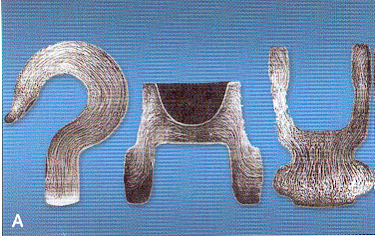
\includegraphics[width=0.5\linewidth]{img/Picture3}
\end{center}

\begin{itemize}
 \item \textbf{Intérêt:} La déformation plastique génère un fibrage qui améliore les performances mécaniques. Ce qui permet de réduire les dimensions, le poids, l'inertie, les vibrations, pour les même efforts.
\end{itemize}
}}

{\frame{
\frametitle{Les classes de forgeage}

Il faut distinguer le \textbf{formage à chaud} et le \textbf{formage à froid}.

Température limite entre formage à froid et formage à chaud:
\begin{itemize}
 \item Aluminium : 193 °C,
 \item Cuivre : 405 °C,
 \item Fer : 631 °C,
 \item Nickel : 590 °C,
 \item Titane : 697 °C.
\end{itemize}
}}

\section{Procédés}

{\frame{
\frametitle{Le formage à chaud: La Forge Libre}

\begin{center}
 \begin{minipage}{0.55\linewidth}
 Le \textbf{forgeage libre} (ou forge libre) est la déformation manuelle d'un lopin métallique à l'aide d'un pilon ou d'un marteau. Il permet d'obtenir à chaud, sans outillages spécifiques, avec des délais courts des pièces unitaires ou des très petites séries. \\ ~\ \\
  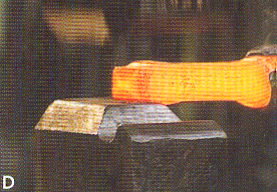
\includegraphics[width=0.9\linewidth]{img/Picture4}
 \end{minipage}\hfill
 \begin{minipage}{0.35\linewidth}
  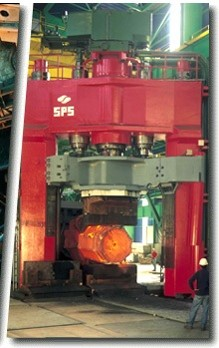
\includegraphics[width=0.9\linewidth]{img/Picture5}
 \end{minipage} 
\end{center}
}}

{\frame{
\frametitle{Estampage / Matriçage}

 \begin{minipage}{0.55\linewidth}
 \begin{itemize}
  \item Formage à chaud par pression ou par chocs de pièces en série, entre deux matrices (outillage spécifique) portant en creux la forme de la pièce,
  \item La précision dimensionnelle est plus grande qu'en forge libre.
  \\ ~\ \\
 \centering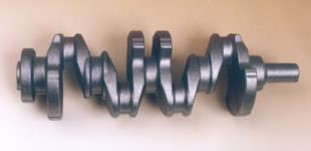
\includegraphics[width=0.9\linewidth]{img/Picture7}
 \end{itemize}
 \end{minipage}\hfill
 \begin{minipage}{0.4\linewidth}
  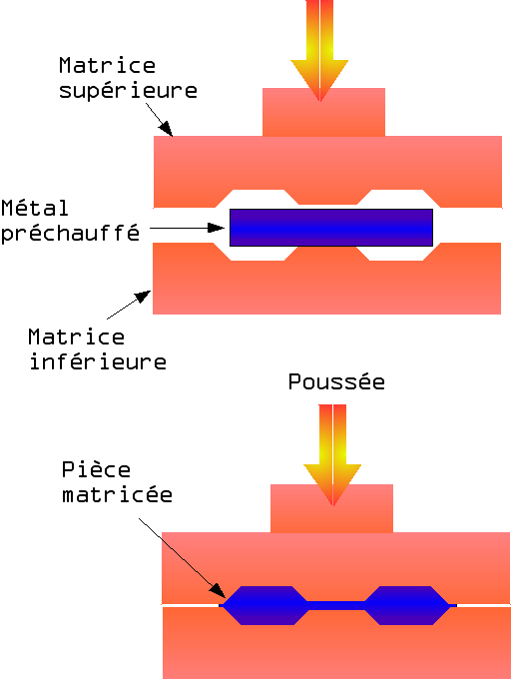
\includegraphics[width=0.9\linewidth]{img/Picture6}
 \end{minipage} 
}}

{\frame{
\frametitle{Estampage / Matriçage}

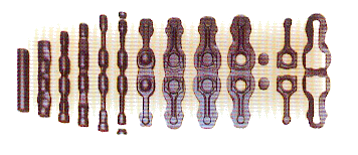
\includegraphics[width=0.9\linewidth]{img/Picture9}\\

 \begin{minipage}{0.55\linewidth}
  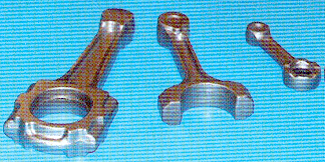
\includegraphics[width=0.9\linewidth]{img/Picture10}
 \end{minipage}\hfill
 \begin{minipage}{0.4\linewidth}
  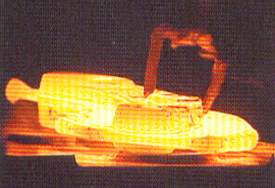
\includegraphics[width=0.9\linewidth]{img/Picture11}
 \end{minipage} 
}}

{\frame{
\frametitle{Filage}

Sous l'action d'un poinçon, cette opération consiste à forcer le métal (ductile) enfermé dans un conteneur à passer au travers d'une filière qui constitue une extrémité de ce dernier. \\ ~\ \\
\begin{minipage}{0.3\linewidth}
 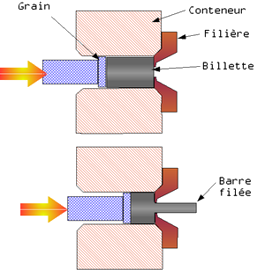
\includegraphics[width=0.9\linewidth]{img/Picture12}
\end{minipage}\hfill
\begin{minipage}{0.3\linewidth}
 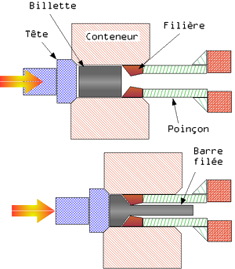
\includegraphics[width=0.9\linewidth]{img/Picture13}
\end{minipage}\hfill
\begin{minipage}{0.3\linewidth}
 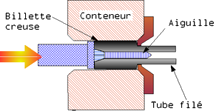
\includegraphics[width=0.9\linewidth]{img/Picture15}
\end{minipage} 
}}

{\frame{
\frametitle{Fluotournage}

Le \textbf{fluotournage} consiste en la déformation plastique de métaux entre un mandrin et une ou plusieurs molettes, entre lesquels la matière « s'écoule », d'où son nom.
 \\ ~\ \\
\centering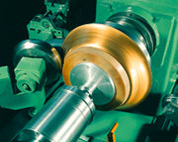
\includegraphics[width=0.5\linewidth]{img/Picture16}
}}

{\frame{
\frametitle{Laminage à chaud}

\begin{minipage}{0.7\linewidth}
Le métal subit une réduction d'épaisseur par écrasement entre les deux cylindres.
\end{minipage}\hfill
\begin{minipage}{0.25\linewidth}
 
\includegraphics[width=0.6\linewidth]{img/Picture17}
\end{minipage}

\begin{itemize}
 \item \textbf{Laminage des produits plats:} Après passage dans un four de réchauffage qui porte les brames à plus de 1000 °C, le métal est acheminé sur des rouleaux motorisés, \\
\centering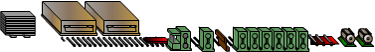
\includegraphics[width=0.7\linewidth]{img/Picture18} \\
\begin{minipage}{0.7\linewidth}
 \item \textbf{Laminage des produits longs:} Un train fil est un train de laminoirs, continu, spécialisé dans la production de fil machine,
\end{minipage}\hfill
\begin{minipage}{0.25\linewidth}
 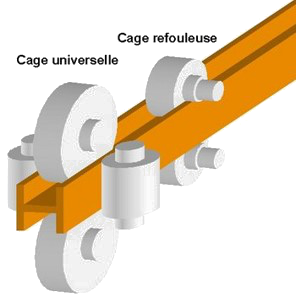
\includegraphics[width=0.8\linewidth]{img/Picture19}
\end{minipage}
\end{itemize}
}}

{\frame{
\frametitle{Formage/frappe à Froid}

\begin{itemize}
 \item Déformation très rapide de pièces longues, visserie, boulonnerie,
 \item Partant d'un morceau de barre ou de fil, il est déformé en l'air ou en matrice fermée pour lui conférer la géométrie visée.
\end{itemize}

\centering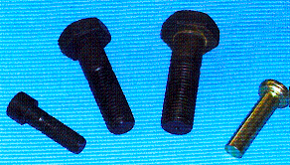
\includegraphics[width=0.5\linewidth]{img/Picture20}
}}

{\frame{
\frametitle{Electrorefoulage}

\begin{itemize}
 \item Le métal est chauffé et déformé localement.
\end{itemize}

\centering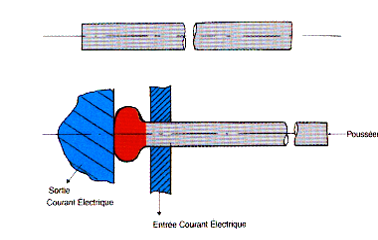
\includegraphics[width=0.5\linewidth]{img/Picture21}
}}

{\frame{
\frametitle{Extrusion}

\begin{minipage}{0.5\linewidth}
\begin{itemize}
 \item L'extrusion est un procédé de fabrication (thermo)mécanique par lequel un matériau compressé est contraint de traverser une filière ayant la section de la pièce à obtenir,
 \item Grandes séries et pièces très précises sans usinage.
\end{itemize}
\end{minipage}\hfill
\begin{minipage}{0.45\linewidth}
 \centering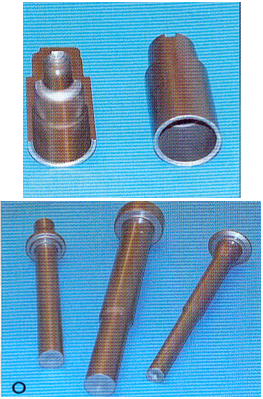
\includegraphics[width=0.6\linewidth]{img/Picture22}
\end{minipage}

\begin{minipage}{0.3\linewidth}
 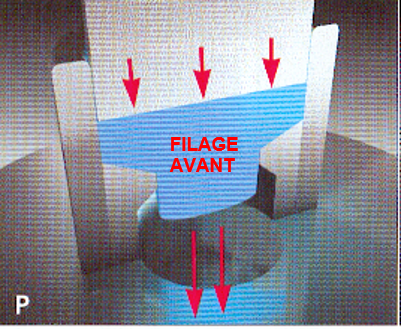
\includegraphics[width=0.9\linewidth]{img/Picture24}
\end{minipage}\hfill
\begin{minipage}{0.3\linewidth}
 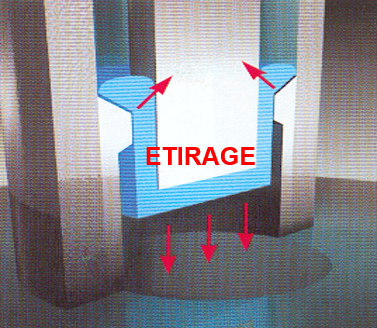
\includegraphics[width=0.9\linewidth]{img/Picture25}
\end{minipage}\hfill
\begin{minipage}{0.3\linewidth}
 
\includegraphics[width=0.9\linewidth]{img/Picture23}
\end{minipage}
}}

{\frame{
\frametitle{Etirage et tréfilage}

\begin{itemize}
 \item Par traction, une barre ou un fil est forcé à passer au travers d'une filière qui réduit sa section,
 \item Le tréfilage est la réduction de la section d'un fil en métal par traction mécanique sur une machine à tréfiler,
 \item Fils électriques, clôtures, câbles, pointes.
\end{itemize}

\centering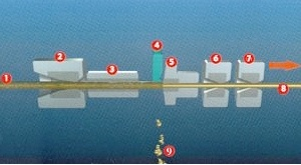
\includegraphics[width=0.4\linewidth]{img/Picture26}
}}

{\frame{
\frametitle{Emboutissage}

\begin{minipage}{0.6\linewidth}
\begin{itemize}
 \item Des produits plats sont conformés par l'action d'un poinçon de forme qui contraint la tôle à épouser la géométrie d'une matrice.
\end{itemize}
\end{minipage}\hfill
\begin{minipage}{0.35\linewidth}
 \centering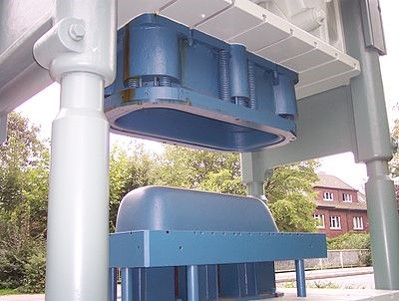
\includegraphics[width=0.7\linewidth]{img/Picture27}
\end{minipage}

\begin{minipage}{0.45\linewidth}
 \centering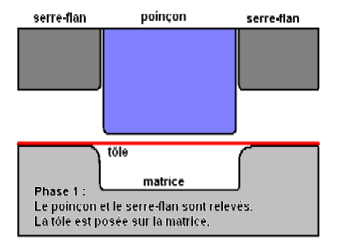
\includegraphics[width=0.7\linewidth]{img/Picture28}
\end{minipage}\hfill
\begin{minipage}{0.45\linewidth}
 \centering
\includegraphics[width=0.7\linewidth]{img/Picture29}
\end{minipage}\\
\begin{minipage}{0.45\linewidth}
 \centering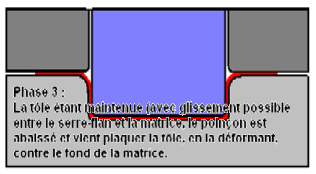
\includegraphics[width=0.7\linewidth]{img/Picture30}
\end{minipage}\hfill
\begin{minipage}{0.45\linewidth}
 \centering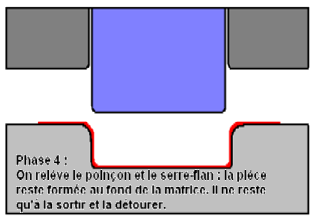
\includegraphics[width=0.7\linewidth]{img/Picture31}
\end{minipage}
}}

\section{Comparaison}

{\frame{
\frametitle{Tableau comparatif}
{\tiny\begin{tabular}{|p{.06\linewidth}|p{.05\linewidth}|p{.065\linewidth}|p{.05\linewidth}|p{.07\linewidth}|p{.06\linewidth}|p{.07\linewidth}|p{.05\linewidth}|p{.08\linewidth}|}
\hline
Procédé & T (°) & Matériaux & Poids & Série & Outillage & Machine & Tolérance (mm) & Suite \\ \hline
Forge libre & 200-400 & Tous & 1kg/200t & 1-50 & Standard & Chocs et pression & 5 & Estampage, Matricage, Usinage \\ \hline
Estampage & 850-1200 & Ferreux & \multirow{2}{*}{\parbox{\linewidth}{50g à 3T}} & \multirow{2}{*}{\parbox{\linewidth}{50-10000/mois}} & \multirow{2}{*}{\parbox{\linewidth}{Matrices spécifiques}} & Chocs & 1-2 & \multirow{2}{*}{\parbox{\linewidth}{Ebavurage, Usinage}} \\ \cline{1-3}\cline{7-8} 
Matriçage & 400-950 & Non Ferreux & & & & Pression & 0.3-0.4 & \\ \hline
Extrusion & A froid & Tous & 50g à 15 kg & 1000 à 5000 p/mois & Spécifiques & Pression  & 0.05-0.1mm (diam) 0,5 (long) & Pas ou peu d'usinage \\
\hline
\end{tabular}}
}}

{\frame{
\frametitle{Conclusion}

\begin{savoir}
Vous êtes capables :
\begin{itemize}
 \item de concevoir une pièce forgée,
 \item de choisir un processus de forgeage.
\end{itemize}
\end{savoir}

\begin{prob}
Vous devez êtes capables :
 \begin{itemize}
 \item de concevoir une pièce moulée.
 \end{itemize}
\end{prob}
}}


\end{document}